\documentclass[write-up.tex]{subfiles}
\begin{document}

\section{Theoretical model}
\subsection{Smoothing Kernel}

Each SPH particle has a circle of influence determined by the Smoothing Kernel $W(r,h)$ where $r$ is the distance from the sample point to the particle center and $h$ is the smoothing radius. The influence of a particle on a sample point increases as the sample point gets closer to the particle center. The choice of smoothing kernel is crucial as it is used by the \hyperlink{Interpolation Equation}{\textbf{Interpolation Equation}} to calculate scalar quantities, such as density. Müller \textit{et al.}\cite{muller} describe two popular smoothing kernels, each with different properties.

\begin{center}
$
    W_{\text{poly}}(r, h) = \displaystyle \frac{315}{64 \pi h^9}
    \begin{cases}
        (h^2-r^2)^3 & 0 \leq r \leq h \\
        0 & \text{otherwise},
    \end{cases}
$
\end{center}

\begin{tikzpicture}
\begin{axis}[
    axis lines = left,
    xlabel = \(r\),
    ylabel = \(W_{poly}(r\text{, }1)\)
]
%Below the red parabola is defined
\addplot [
    domain=0:1,
    samples=200,
    color=cyan,
]
{315/(64 * 3.14159) * (1-x^2)^3};
\end{axis}
\end{tikzpicture}

$W_{\text{poly}}(r, h)$ is a versatile kernel designed to simplify distance computations by squaring the distance term, eliminating the need for square root calculations when using the Pythagorean Theorem. However, Müller \textit{et al.}\cite{muller} note that when $W_{\text{poly}}(r, h)$ is used for pressure computations, as required for enforcing incompressibility in this project, particles tend to cluster due to the gradient's effect on pressure calculation. The gradient of $W_{\text{poly}}(r, h)$ approaches zero for small distances, resulting in a diminishing repulsion force.

\begin{center}
$
    W_{\text{spiky}}(r, h) = \displaystyle \frac{15}{\pi h^6}
    \begin{cases}
        (h-r)^3 & 0 \leq r \leq h \\
        0 & \text{otherwise},
    \end{cases}
$
\end{center}

\begin{tikzpicture}
\begin{axis}[
    axis lines = left,
    xlabel = \(r\),
    ylabel = \(W_{spiky}(r\text{, }1)\)
]
%Below the red parabola is defined
\addplot [
    domain=0:1,
    samples=200,
    color=cyan,
]
{15/3.14159 * (1-x)^3};
\end{axis}
\end{tikzpicture}

$W_{\text{spiky}}(r, h)$ is used specifically for pressure computations. Its gradient is high when $r$ is close to $0$, generating the required repulsion forces for pressure calculations and therefore making it the superior choice for my simulation. Note that for the simulation, the influence value returned will also be divided by the volume of our kernel, this keeps values consistent regardless of our values of $h$.


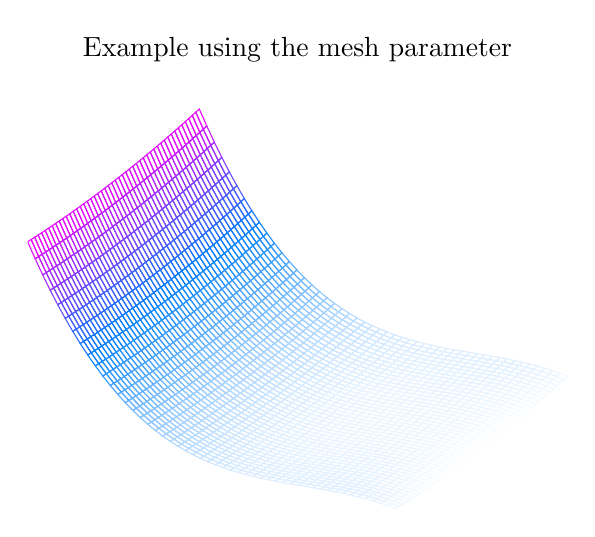
\begin{tikzpicture}
\begin{axis}[
    title=Example using the mesh parameter,
    hide axis,
    colormap/cool,
]
\addplot3[
    mesh,
    samples=50,
    domain=-2:2,
]
{15/3.14 * (1-x)^3 +y^2};
\end{axis}
\end{tikzpicture}

\subsection{Interpolation Equation}
The Interpolation Equation is responsible for calculating a scalar quantity $A$ at a location $r$ by a weighted sum of contributions from all the particles within our simulation. This is given by:



\end{document}
